\begin{center}
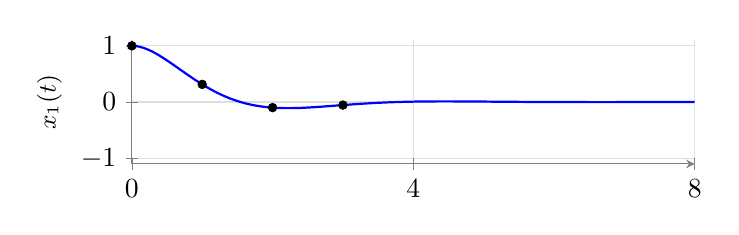
\begin{tikzpicture}
\begin{axis}[
  width=0.72\linewidth, height=0.26\linewidth,
  ylabel={$x_1(t)$},
  axis lines=left,
  axis line style={gray},
  label style={font=\small},
  xmin=0, xmax=8, ymin=-1.1, ymax=1.1,
  xtick={0,4,8}, ytick={-1,0,1},
  grid=major, grid style={gray!25},
]
\addplot[domain=0:8, samples=200, thick, blue]
  {exp(-x)*(cos(deg(sqrt(2)*x)) + (1/sqrt(2))*sin(deg(sqrt(2)*x)))};
\addplot[only marks, mark=*, mark size=1.5pt, black]
  coordinates {(0,1) (1,0.314) (2,-0.099) (3,-0.054)};
\end{axis}
\end{tikzpicture}

\vspace{0.7em}

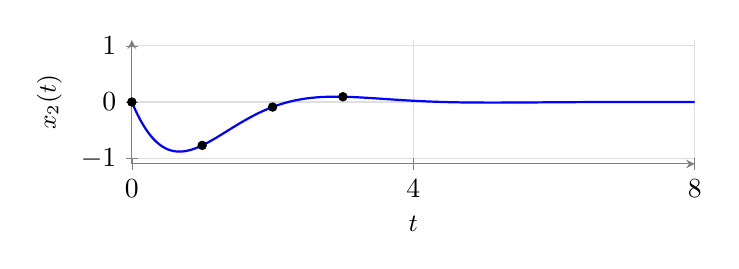
\begin{tikzpicture}
\begin{axis}[
  width=0.72\linewidth, height=0.26\linewidth,
  xlabel={$t$}, ylabel={$x_2(t)$},
  axis lines=left,
  axis line style={gray},
  label style={font=\small},
  xmin=0, xmax=8, ymin=-1.1, ymax=1.1,
  xtick={0,4,8}, ytick={-1,0,1},
  grid=major, grid style={gray!25},
]
\addplot[domain=0:8, samples=200, thick, blue]
  {-(3/sqrt(2))*exp(-x)*sin(deg(sqrt(2)*x))};
\addplot[only marks, mark=*, mark size=1.5pt, black]
  coordinates {(0,0) (1,-0.771) (2,-0.089) (3,0.094)};
\end{axis}
\end{tikzpicture}
\end{center}
